\documentclass{standalone}
\usepackage{tikz}
\usepackage{pgfplots}

\pgfplotsset{compat=1.17}

\begin{document}

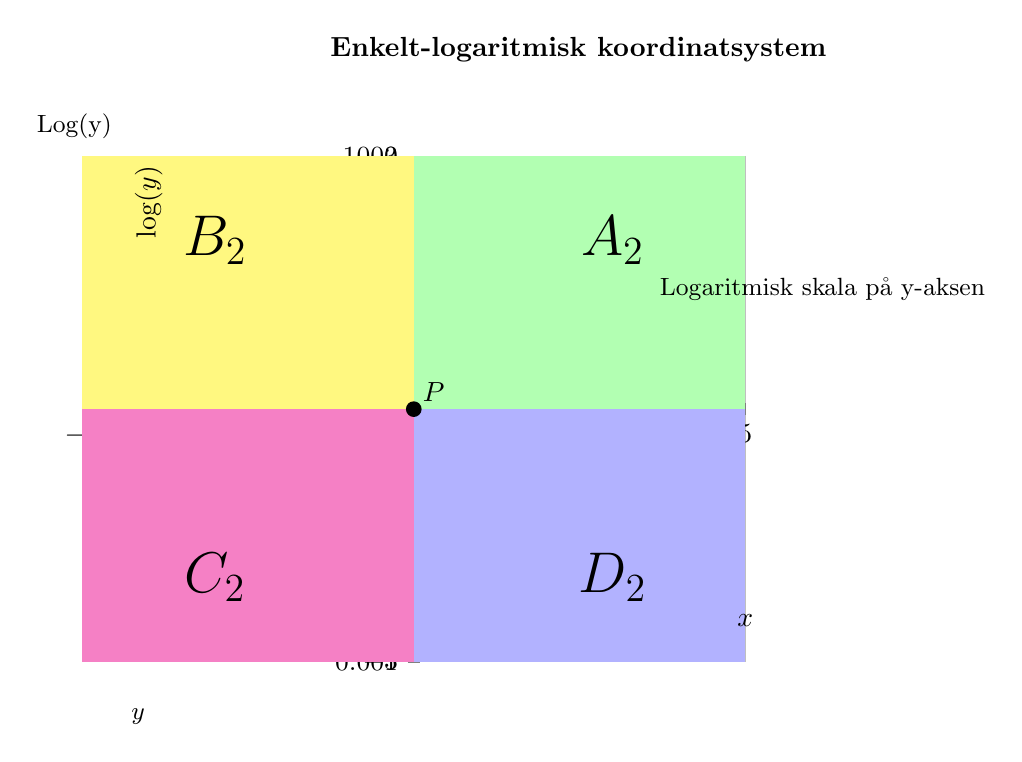
\begin{tikzpicture}
    \begin{axis}[
        width=10cm, height=8cm, % Adjusted size to avoid dimension issues
        axis lines=middle,
        xlabel={$x$},
        ylabel={$\log(y)$},
        xmin=-5, xmax=5,
        ymin=-3, ymax=3,
        xtick={-5,-4,...,5},
        ytick={-3,-2,...,3},
        xlabel near ticks,
        ylabel near ticks,
        extra y ticks={-3,-2,-1,0,1,2,3},
        extra y tick labels={0.001, 0.01, 0.1, 1, 10, 100, 1000},
        grid=both,
        minor tick num=1,
        axis line style={-stealth},
        xlabel style={at={(1,0.05)}, anchor=south},
        ylabel style={at={(0.1,1)}, anchor=east},
        enlargelimits=false,
        clip=false,
        every axis plot/.append style={thick}
    ]

    % Filling the regions with colors
    \addplot [draw=none, fill=green!30] coordinates { (0,0) (5,0) (5,3) (0,3) };
    \addplot [draw=none, fill=yellow!50] coordinates { (0,0) (-5,0) (-5,3) (0,3) };
    \addplot [draw=none, fill=magenta!50] coordinates { (0,0) (-5,0) (-5,-3) (0,-3) };
    \addplot [draw=none, fill=blue!30] coordinates { (0,0) (5,0) (5,-3) (0,-3) };
    
    % Drawing the point P
    \node at (axis cs: 0,0) [circle,fill=black,inner sep=2pt] {};
    \node at (axis cs: 0.3,0.2) {$P$};
    
    % Labels for each quadrant
    \node at (axis cs: 3,2) {\huge $A_2$};
    \node at (axis cs: -3,2) {\huge $B_2$};
    \node at (axis cs: -3,-2) {\huge $C_2$};
    \node at (axis cs: 3,-2) {\huge $D_2$};

    \end{axis}
    
    % Title and Y-axis label
    \node[anchor=south] at (6.3,7.5) {\textbf{Enkelt-logaritmisk koordinatsystem}};
    \node[anchor=north] at (9.4,5.0) {\small Logaritmisk skala på y-aksen};
    \node[anchor=east] at (0.5,6.8) {\small Log(y)};
    \node[anchor=west] at (0.5,-0.7) {\small $y$};
\end{tikzpicture}

\end{document}
